\documentclass[11pt,preprint, authoryear]{elsarticle}

\usepackage{lmodern}
%%%% My spacing
\usepackage{setspace}
\setstretch{1.2}
\DeclareMathSizes{12}{14}{10}{10}

% Wrap around which gives all figures included the [H] command, or places it "here". This can be tedious to code in Rmarkdown.
\usepackage{float}
\let\origfigure\figure
\let\endorigfigure\endfigure
\renewenvironment{figure}[1][2] {
    \expandafter\origfigure\expandafter[H]
} {
    \endorigfigure
}

\let\origtable\table
\let\endorigtable\endtable
\renewenvironment{table}[1][2] {
    \expandafter\origtable\expandafter[H]
} {
    \endorigtable
}


\usepackage{ifxetex,ifluatex}
\usepackage{fixltx2e} % provides \textsubscript
\ifnum 0\ifxetex 1\fi\ifluatex 1\fi=0 % if pdftex
  \usepackage[T1]{fontenc}
  \usepackage[utf8]{inputenc}
\else % if luatex or xelatex
  \ifxetex
    \usepackage{mathspec}
    \usepackage{xltxtra,xunicode}
  \else
    \usepackage{fontspec}
  \fi
  \defaultfontfeatures{Mapping=tex-text,Scale=MatchLowercase}
  \newcommand{\euro}{€}
\fi

\usepackage{amssymb, amsmath, amsthm, amsfonts}

\def\bibsection{\section*{References}} %%% Make "References" appear before bibliography


\usepackage[round]{natbib}

\usepackage{longtable}
\usepackage[margin=2.3cm,bottom=2cm,top=2.5cm, includefoot]{geometry}
\usepackage{fancyhdr}
\usepackage[bottom, hang, flushmargin]{footmisc}
\usepackage{graphicx}
\numberwithin{equation}{section}
\numberwithin{figure}{section}
\numberwithin{table}{section}
\setlength{\parindent}{0cm}
\setlength{\parskip}{1.3ex plus 0.5ex minus 0.3ex}
\usepackage{textcomp}
\renewcommand{\headrulewidth}{0.2pt}
\renewcommand{\footrulewidth}{0.3pt}

\usepackage{array}
\newcolumntype{x}[1]{>{\centering\arraybackslash\hspace{0pt}}p{#1}}

%%%%  Remove the "preprint submitted to" part. Don't worry about this either, it just looks better without it:
\makeatletter
\def\ps@pprintTitle{%
  \let\@oddhead\@empty
  \let\@evenhead\@empty
  \let\@oddfoot\@empty
  \let\@evenfoot\@oddfoot
}
\makeatother

 \def\tightlist{} % This allows for subbullets!

\usepackage{hyperref}
\hypersetup{breaklinks=true,
            bookmarks=true,
            colorlinks=true,
            citecolor=blue,
            urlcolor=blue,
            linkcolor=blue,
            pdfborder={0 0 0}}


% The following packages allow huxtable to work:
\usepackage{siunitx}
\usepackage{multirow}
\usepackage{hhline}
\usepackage{calc}
\usepackage{tabularx}
\usepackage{booktabs}
\usepackage{caption}


\newenvironment{columns}[1][]{}{}

\newenvironment{column}[1]{\begin{minipage}{#1}\ignorespaces}{%
\end{minipage}
\ifhmode\unskip\fi
\aftergroup\useignorespacesandallpars}

\def\useignorespacesandallpars#1\ignorespaces\fi{%
#1\fi\ignorespacesandallpars}

\makeatletter
\def\ignorespacesandallpars{%
  \@ifnextchar\par
    {\expandafter\ignorespacesandallpars\@gobble}%
    {}%
}
\makeatother

\newlength{\cslhangindent}
\setlength{\cslhangindent}{1.5em}
\newenvironment{CSLReferences}%
  {\setlength{\parindent}{0pt}%
  \everypar{\setlength{\hangindent}{\cslhangindent}}\ignorespaces}%
  {\par}


\urlstyle{same}  % don't use monospace font for urls
\setlength{\parindent}{0pt}
\setlength{\parskip}{6pt plus 2pt minus 1pt}
\setlength{\emergencystretch}{3em}  % prevent overfull lines
\setcounter{secnumdepth}{5}

%%% Use protect on footnotes to avoid problems with footnotes in titles
\let\rmarkdownfootnote\footnote%
\def\footnote{\protect\rmarkdownfootnote}
\IfFileExists{upquote.sty}{\usepackage{upquote}}{}

%%% Include extra packages specified by user

%%% Hard setting column skips for reports - this ensures greater consistency and control over the length settings in the document.
%% page layout
%% paragraphs
\setlength{\baselineskip}{12pt plus 0pt minus 0pt}
\setlength{\parskip}{12pt plus 0pt minus 0pt}
\setlength{\parindent}{0pt plus 0pt minus 0pt}
%% floats
\setlength{\floatsep}{12pt plus 0 pt minus 0pt}
\setlength{\textfloatsep}{20pt plus 0pt minus 0pt}
\setlength{\intextsep}{14pt plus 0pt minus 0pt}
\setlength{\dbltextfloatsep}{20pt plus 0pt minus 0pt}
\setlength{\dblfloatsep}{14pt plus 0pt minus 0pt}
%% maths
\setlength{\abovedisplayskip}{12pt plus 0pt minus 0pt}
\setlength{\belowdisplayskip}{12pt plus 0pt minus 0pt}
%% lists
\setlength{\topsep}{10pt plus 0pt minus 0pt}
\setlength{\partopsep}{3pt plus 0pt minus 0pt}
\setlength{\itemsep}{5pt plus 0pt minus 0pt}
\setlength{\labelsep}{8mm plus 0mm minus 0mm}
\setlength{\parsep}{\the\parskip}
\setlength{\listparindent}{\the\parindent}
%% verbatim
\setlength{\fboxsep}{5pt plus 0pt minus 0pt}



\begin{document}



\begin{frontmatter}  %

\title{Time-varying Correlation of South African Property Stocks and the
ALSI}

% Set to FALSE if wanting to remove title (for submission)




\author[Add1]{Andrew Hyde}
\ead{23365935@sun.ac.za}





\address[Add1]{Stellenbosch University, South Africa}


\begin{abstract}
\small{
This analysis of the current yield spreads in the local bond market
places the current high spreads into historical context.
}
\end{abstract}

\vspace{1cm}





\vspace{0.5cm}

\end{frontmatter}



%________________________
% Header and Footers
%%%%%%%%%%%%%%%%%%%%%%%%%%%%%%%%%
\pagestyle{fancy}
\chead{}
\rhead{}
\lfoot{}
\rfoot{\footnotesize Page \thepage}
\lhead{}
%\rfoot{\footnotesize Page \thepage } % "e.g. Page 2"
\cfoot{}

%\setlength\headheight{30pt}
%%%%%%%%%%%%%%%%%%%%%%%%%%%%%%%%%
%________________________

\headsep 35pt % So that header does not go over title




\hypertarget{introduction}{%
\section{\texorpdfstring{Introduction
\label{Introduction}}{Introduction }}\label{introduction}}

\hypertarget{data-and-methodology}{%
\section{\texorpdfstring{Data and Methodology
\label{Methodology}}{Data and Methodology }}\label{data-and-methodology}}

\hypertarget{data}{%
\subsection{Data}\label{data}}

The dataset used in this study is the ALSI returns data from 2005 to
2022, which included both traditional equities and REITs. Investigation
into the data reveals that there are four unique sectors in the data,
namely; Financials, Industrials, Resources and Property. There are
missing values present in the dataset.

Given that the objective of this study is to explore the time varying
correlation between the ALSI equities and REITs missing data poses a
problem. To address this concern, the dataset is separated into two
groups, one group for ALSI equities and the other for REITs. Next, the
problem of missing values is dealt with by imputing values for both
groups separately.

Separating the data into two groups, before imputing values, is done to
preserve the properties and distribution elements of the ALSI returns
and REIT returns. With that in mind, missing values for the ALSI
equities are imputed using returns distribution draw from the collective
ALSI group less REITs. Missing values for each REIT equity are imputed
using the returns distribution of that equity. This is done to enable
analysis of correlation between REITS, as well as with the rest of the
ALSI equities. The code used in this section follows a practical covered
in Financial Econometrics 871 (Katzke, 2022b).

Figure 2.1 displays the available data for each REIT. Based on
availability of data the following REITs are selected: Capital \&
Counties Properties PLC, Emira Property Fund Limited, Hyprop Investments
Limited, Growthpoint Properties Limited, Resilient Reit Limited,
Redefine Properties Limited and SA Corporate Real Estate Limited.

Given that this analysis is conducted to explore the time-varying
correlation relationships of equity pairs, returns data is log
transformed and mean scaled so that the data used conforms to a normal
distribution centered around its mean. This is especially important as
this allows one to make inferences based on statistical assumptions.

\begin{figure}
\centering
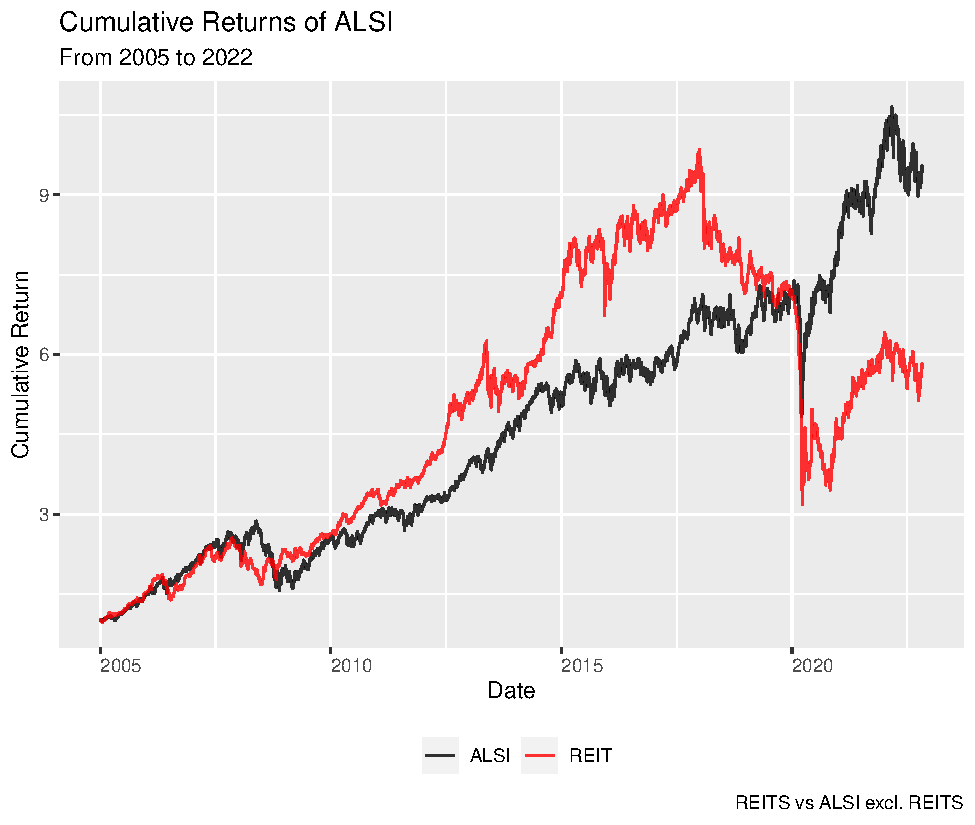
\includegraphics{Fin_Metrics_Project_files/figure-latex/unnamed-chunk-1-1.pdf}
\caption{REITs Dataset}
\end{figure}

\hypertarget{methodology}{%
\subsection{Methodology}\label{methodology}}

A Dynamic Conditional Correlation Generalized AutoRegressive Conditional
Heteroskedasticity (DCC GARCH) model is used to perform this analysis.
This model allows for the estimation of time-varying conditional
correlation structures that are noise reduced, taking the GARCH(1,1)
model further by allowing for multivariate volatility modeling (Engle,
2002; Katzke, 2022d).

The DCC model makes use of non-Linear combinations of univariate GARCH
models to directly model the correlations as a dynamic time-varying
process i.e.~estimating the conditional correlation matrix directly
(Engle, 2002)

The DCC GARCH model follows a two-step approach.

\hypertarget{step-one}{%
\subsubsection{Step One}\label{step-one}}

Estimates are obtained by fitting a univariate GARCH(1,1) model to the
residuals of the vector autoregression (VAR) using the combined imputed
data. The VAR allows for the examination of relationships between series
over time and the residuals it produces \(\alpha_{t}\) can be broken
down into the structural volatility component \(z_{t}\) and the noise
component \(\mu_{t}\), provided \(\alpha_{t}\) are white noise
errors/residuals Katzke, 2022c).

The DCC GARCH model is defined as follows:

\[
H_{t}=D_{t}. R_{t}. D_{t},
\]

where \(H_{t}\) is positive definite variance-covariance matrix which is
splits into identical diagonal matrices \(D_{t}\) and \(R_{t}\), the
time-varying correlation estimates. The estimation of \(R_{T}\) requires
it to be inverted at each estimated period, therefore a proxy similar to
a GARCH(1,1), denoted by \(Q_{i j, t}\), is to be used (Engle, 2002).

\[
\begin{aligned}
Q_{i j, t} & =\bar{Q}+a\left(z_{t-1} z_{t-1}^{\prime}-\bar{Q}\right)+b\left(Q_{i j, t-1}-\bar{Q}\right) \\
& =(1-a-b) \bar{Q}+a z_{t-1} z_{t-1}^{\prime}+b . Q_{i j, t-1}
\end{aligned}
\]

Where \(Q_{i j, t}\) the unconditional (sample) variance estimate
between series \(i\) and \(j\), and \(\bar{Q}\) is the unconditional
matrix of standardized residuals from each univariate pair estimate.

The following equation is used to estimate \(R_{t}\):

\[
R_{t}=\operatorname{diag}\left(Q_{t}\right)^{-1 / 2} Q_{t} . \operatorname{diag}\left(Q_{t}\right)^{-1 / 2} .
\]

Which has bivariate elements:

\[
R_{t}=\rho_{i j, t}=\frac{q_{i, j, t}}{\sqrt{q_{i i, t} \cdot q_{j j, t}}}
\]

The resulting DCC model is then formulated as:

\[
\begin{aligned}
\varepsilon_{t} & \sim N\left(0, D_{t} \cdot R_{t} \cdot D_{t}\right) \\
D_{t}^{2} & \sim \text { Univariate GARCH }(1,1) \text { processes } \forall(\mathrm{i}, \mathrm{j}), \mathrm{i} \neq \mathrm{j} \\
z_{t} & =D_{t}^{-1} \cdot \varepsilon_{t} \\
Q_{t} & =\bar{Q}(1-a-b)+a\left(z_{t}^{\prime} z_{t}\right)+b\left(Q_{t-1}\right) \\
R_{t} & =\operatorname{Diag}\left(Q_{t}^{-1}\right) \cdot Q_{t} . \operatorname{Diag}\left(Q_{t}{ }^{-1}\right)
\end{aligned}
\]

\hypertarget{step-two}{%
\subsubsection{Step Two}\label{step-two}}

Using the standardized residuals from step one, the dynamic,
time-varying conditional correlations estimates can be obtained using a
log-likelihood approach.

The volatility approximation series that is estimated \(H_{t}\), can
then be standardized and used in fitting a DCC model for \(\eta_{t}\)
(Katzke, 2022c).

\[
\eta_{i, t}=\frac{\hat{\alpha_{i, t}}}{\hat{\sigma_{i, t}}}
\] The DDC GARCH model is run twice. The first iteration models the
time-varying conditional correlation structure between the ALSI and
REITs, as well as the time-varying correlation structure between the
seven individual REITs included in the study.The second applies a
stratification method to the data before the DCC GARCH model is re-run.
The stratification methods enables one to examine how these time-varying
conditional correlation structure change in periods of low and high
volatility.

The stratification technique is used to isolate return dates when South
African markets experienced high levels of volatility. To do this, the
South African Rand is used as a benchmark index and is filtered for its
own top and bottom decile quantile (10\%) by monthly standard deviation
of Rand volatility. These dates are then used to filter the
ALSI\_returns into dates with low and high volatility. The code used in
this section follows a practical covered in Financial Econometrics 871
(Katzke, 2022a).

Following the stratification, the time-varying conditional correlation
structure is mapped between Capital \& Counties Properties PLC
(Capco/CCO) and both the ALSI and other SA listed REITs. This section
further explores the relationship between Capital \& Counties Properties
PLC, a UK based REIT and Redefine Properties Limited, an SA based REIT,
whom are both listed on the JSE.

\hypertarget{results-and-discussion}{%
\section{\texorpdfstring{Results and Discussion
\label{Results}}{Results and Discussion }}\label{results-and-discussion}}

\hypertarget{time-varying-correlation-reits-and-alsi}{%
\subsection{Time-varying Correlation: REITs and
ALSI}\label{time-varying-correlation-reits-and-alsi}}

\begin{figure}
\centering
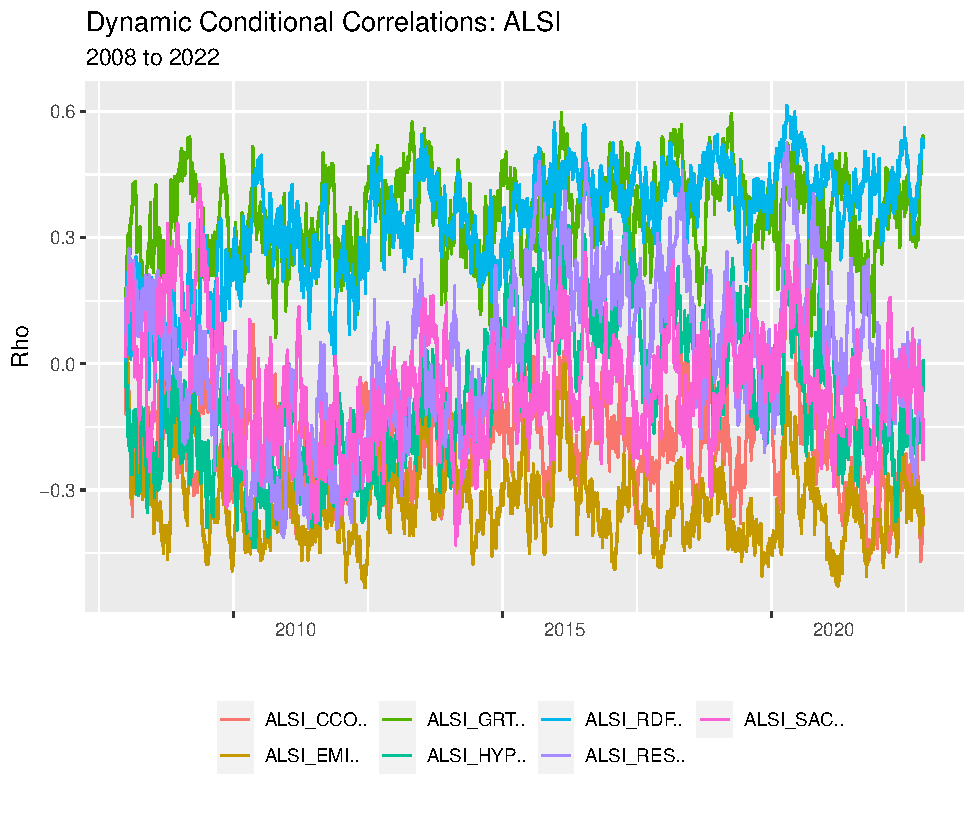
\includegraphics{Fin_Metrics_Project_files/figure-latex/unnamed-chunk-4-1.pdf}
\caption{Dynamic Conditional Correlations Graph}
\end{figure}

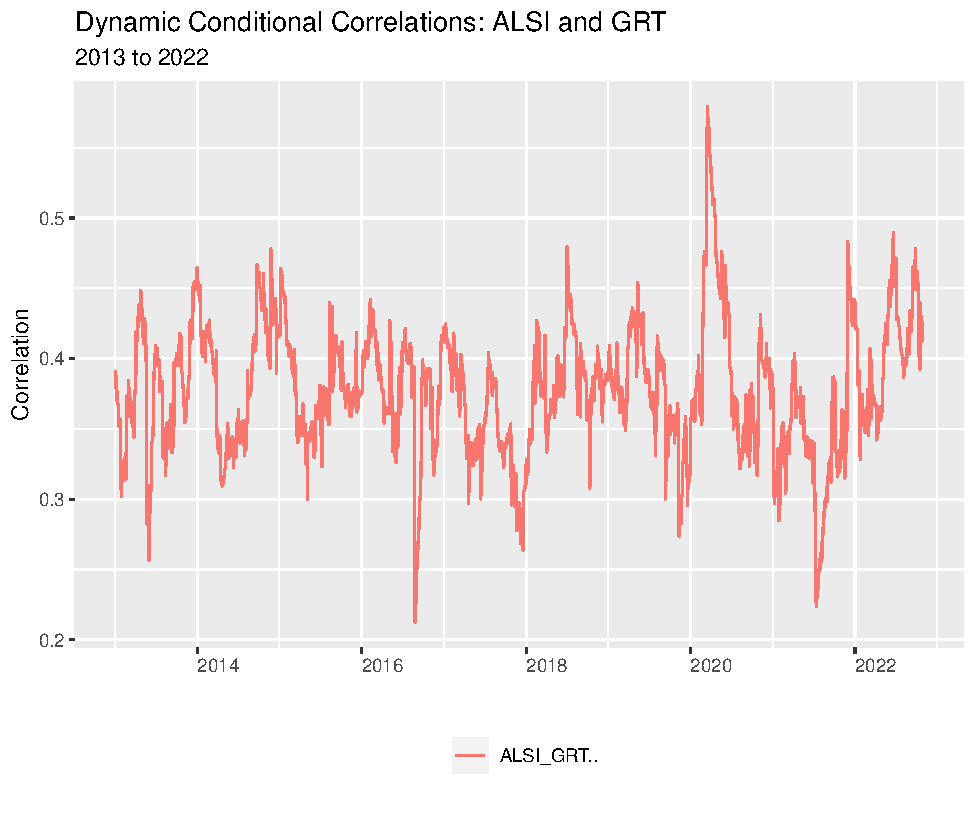
\includegraphics[width=0.5\linewidth]{Fin_Metrics_Project_files/figure-latex/figures-side-1}
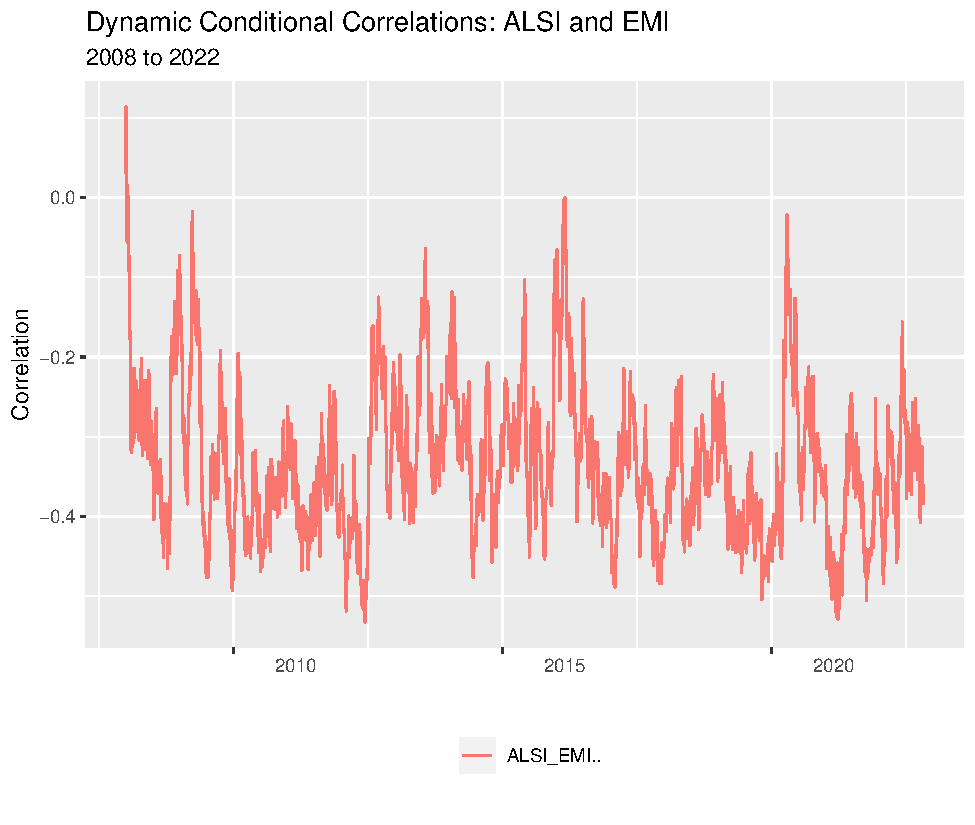
\includegraphics[width=0.5\linewidth]{Fin_Metrics_Project_files/figure-latex/figures-side-2}
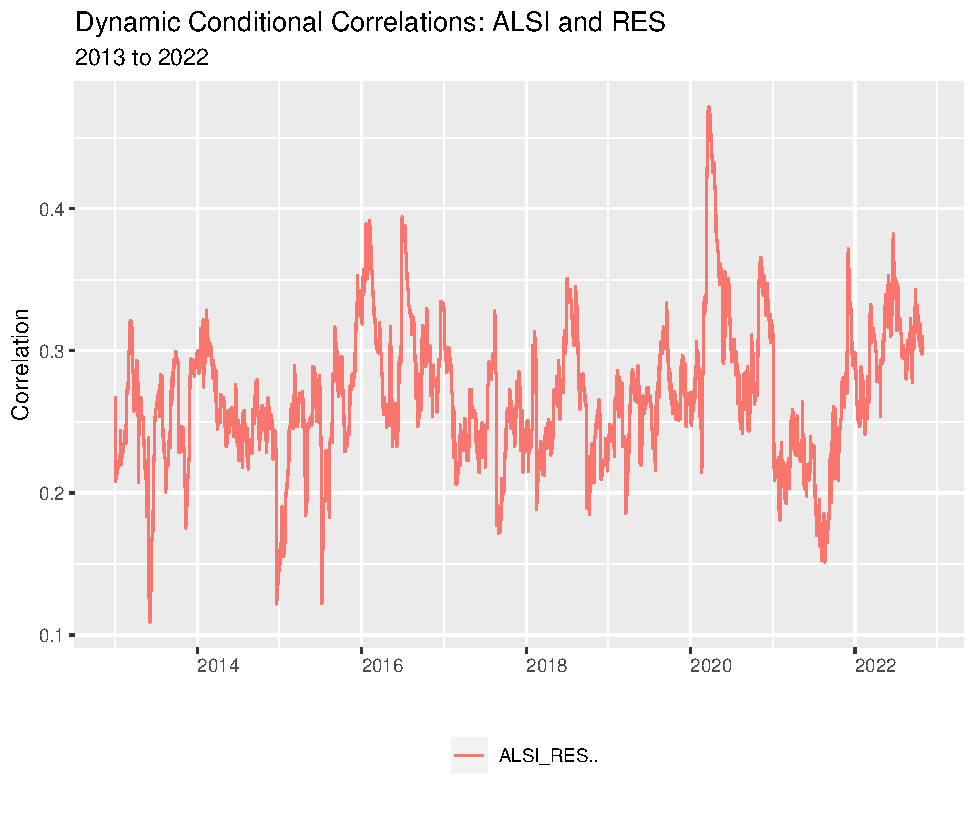
\includegraphics[width=0.5\linewidth]{Fin_Metrics_Project_files/figure-latex/figures-side-3}
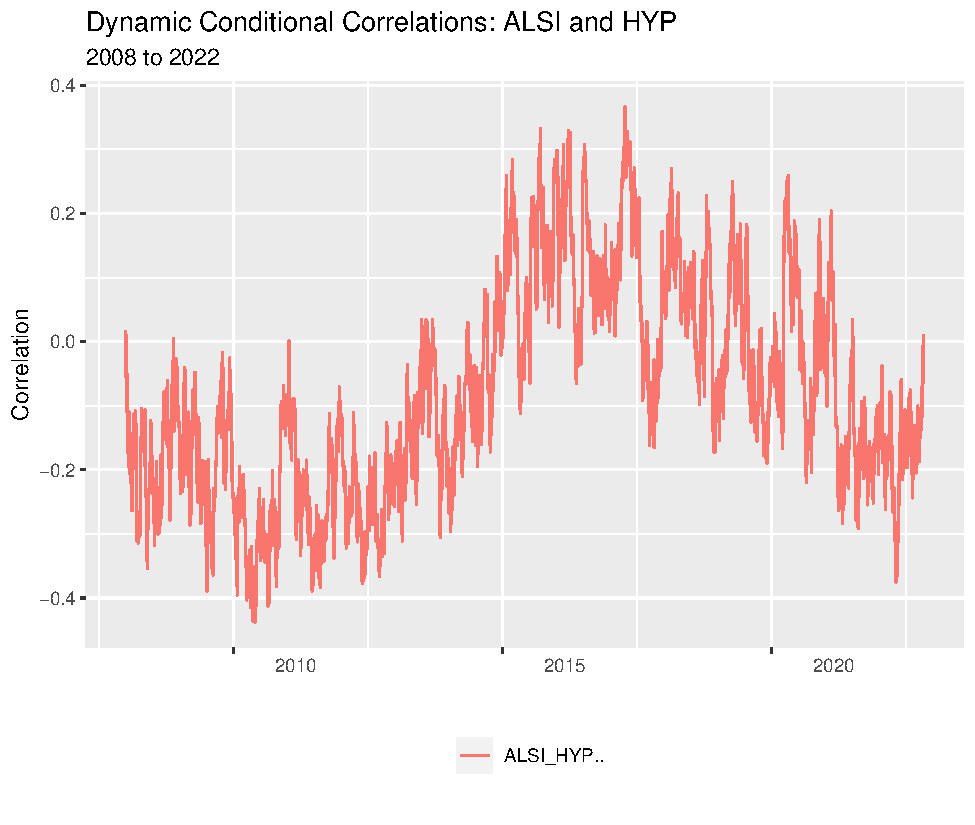
\includegraphics[width=0.5\linewidth]{Fin_Metrics_Project_files/figure-latex/figures-side-4}
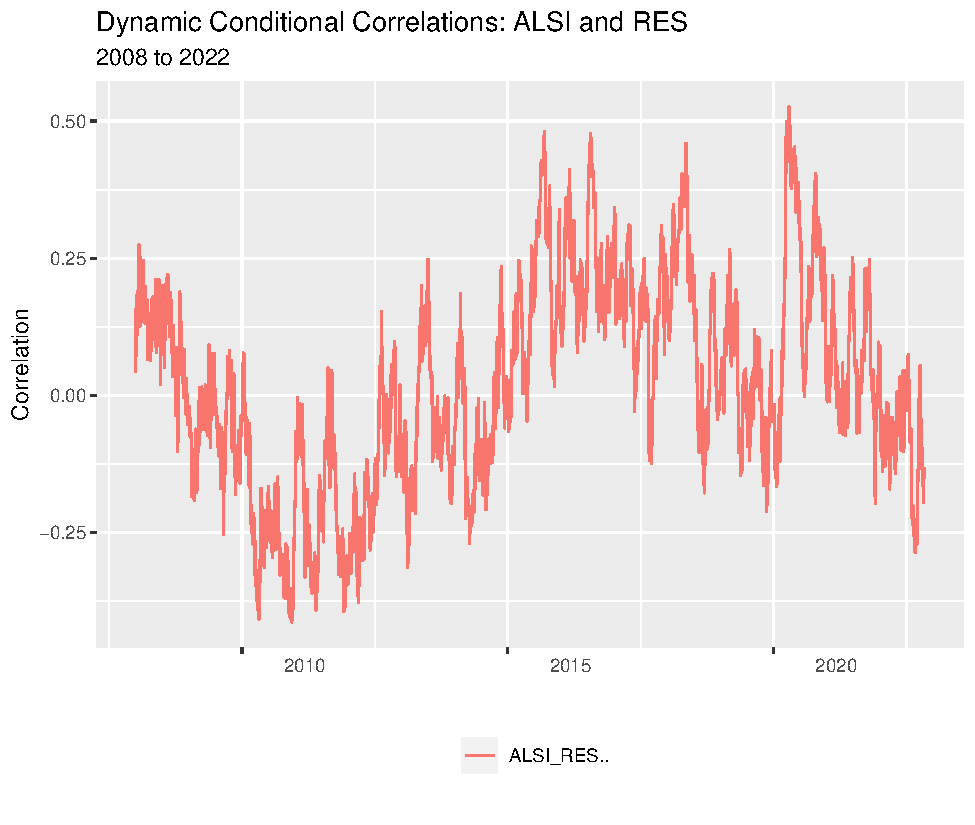
\includegraphics[width=0.5\linewidth]{Fin_Metrics_Project_files/figure-latex/figures-side-5}
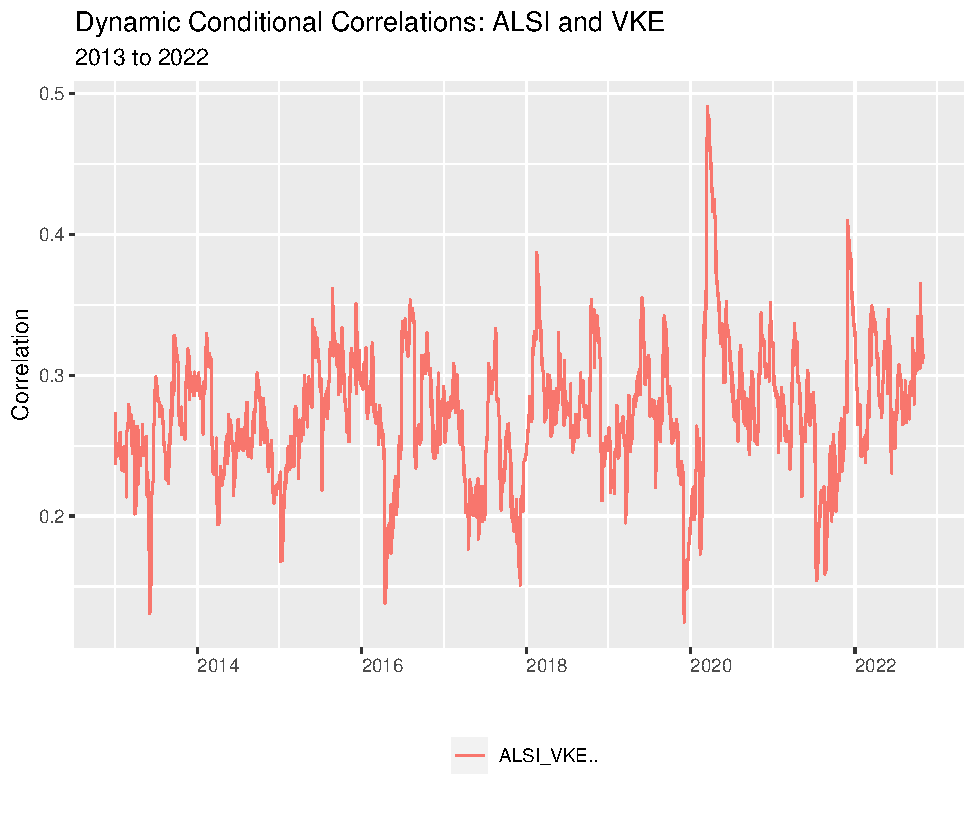
\includegraphics[width=0.5\linewidth]{Fin_Metrics_Project_files/figure-latex/figures-side-6}
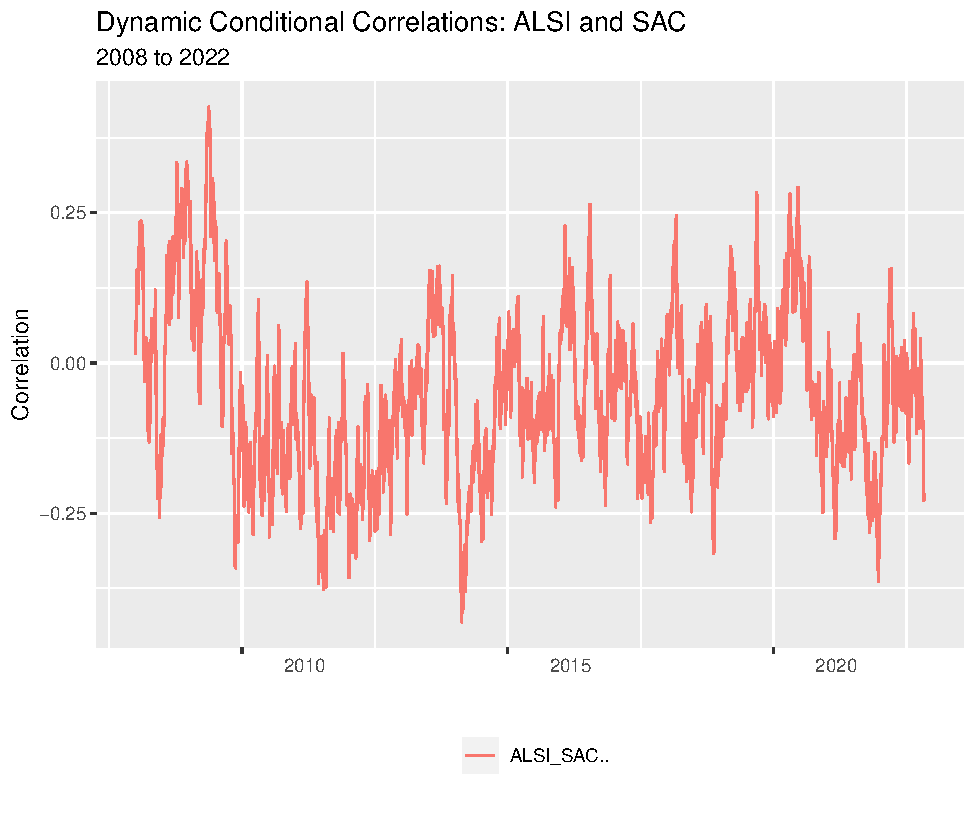
\includegraphics[width=0.5\linewidth]{Fin_Metrics_Project_files/figure-latex/figures-side-7}

\hypertarget{time-varying-correlation-periods-of-high-and-low-volatility}{%
\subsection{Time-varying Correlation: Periods of High and Low
Volatility}\label{time-varying-correlation-periods-of-high-and-low-volatility}}

In this section, periods of high USD/ZAR (Dollar Rand) volatility are
isolated and used as to filter for the ALSI combined and imputed data.
The premise being that periods of high Rand volatility can act as an
indicator for high levels of volatility in South Africa financial
markets and other asset classes. These highly volatile periods are then
used as an index to filter the returns data for periods where South
African markets were volatile.

Given that the high volatility combine imputed ALSI returns data will
have large missing gaps due to periods of moderate or low volatility,
dynamic correlations between equity pairs will have to be charted for
short periods of a time. This is due to the fact that the graphing
function used will not skip whole year periods.

Following this methodology of running multiple DCC models on smaller
periods of high volatility decreases the run time of the model.

\begin{figure}
\centering
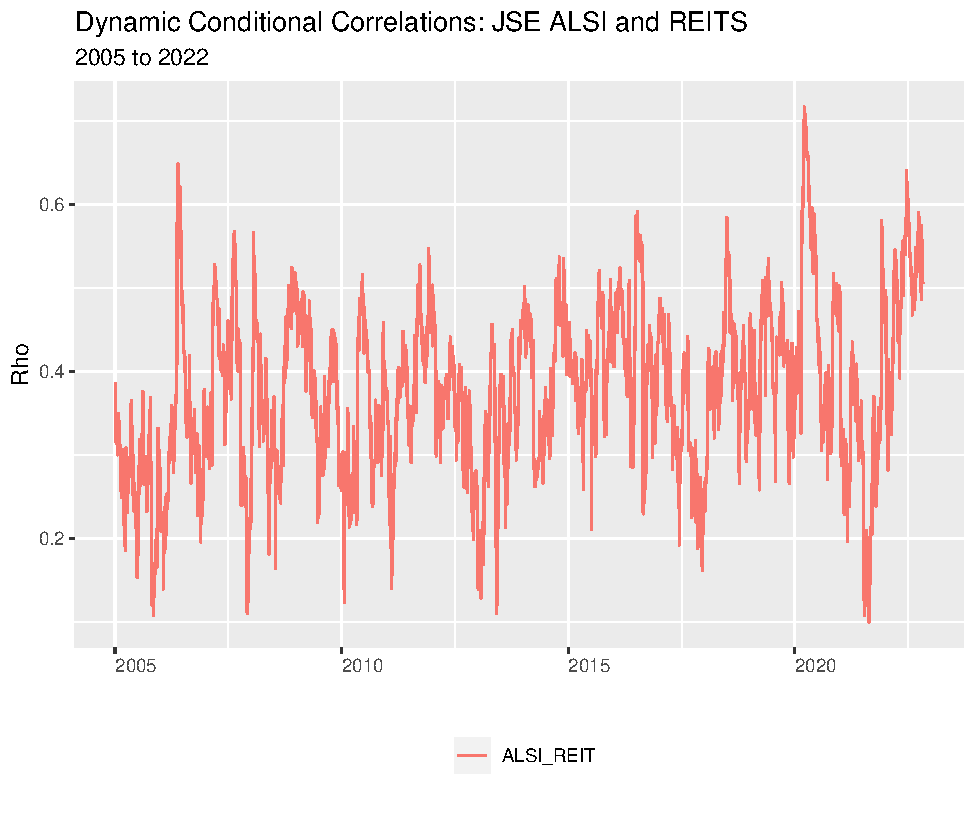
\includegraphics{Fin_Metrics_Project_files/figure-latex/unnamed-chunk-6-1.pdf}
\caption{Dynamic Conditional Correlations Graph}
\end{figure}

\begin{figure}
\centering
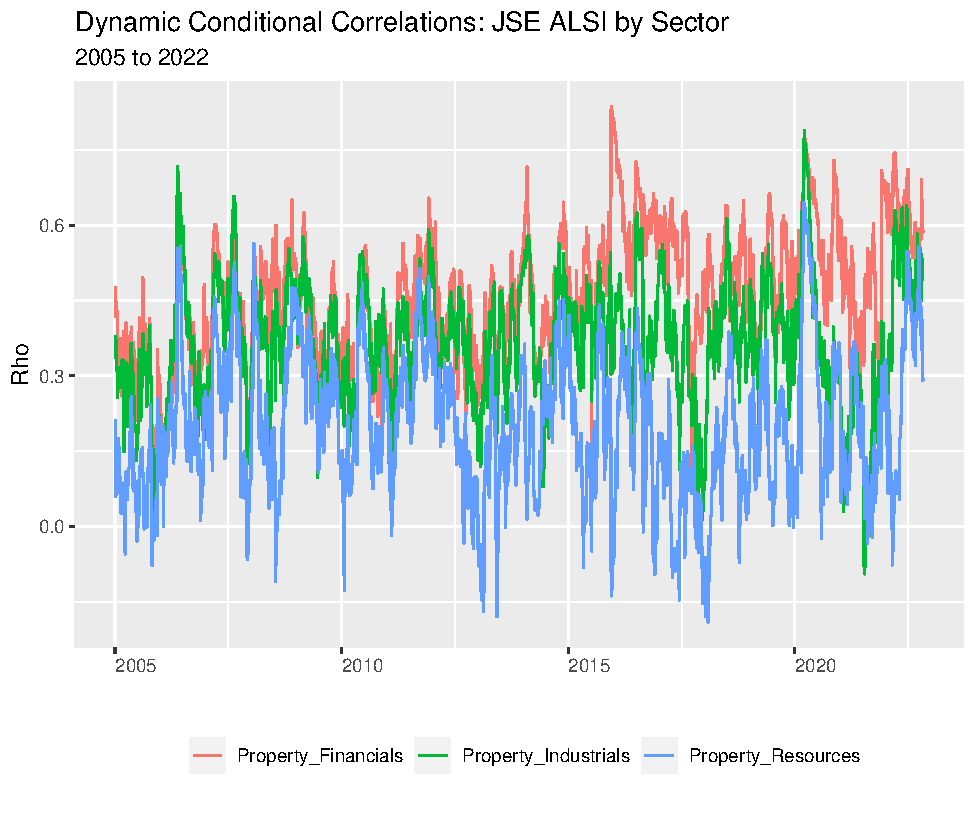
\includegraphics{Fin_Metrics_Project_files/figure-latex/unnamed-chunk-8-1.pdf}
\caption{Dynamic Conditional Correlations Graph}
\end{figure}

\begin{figure}
\centering
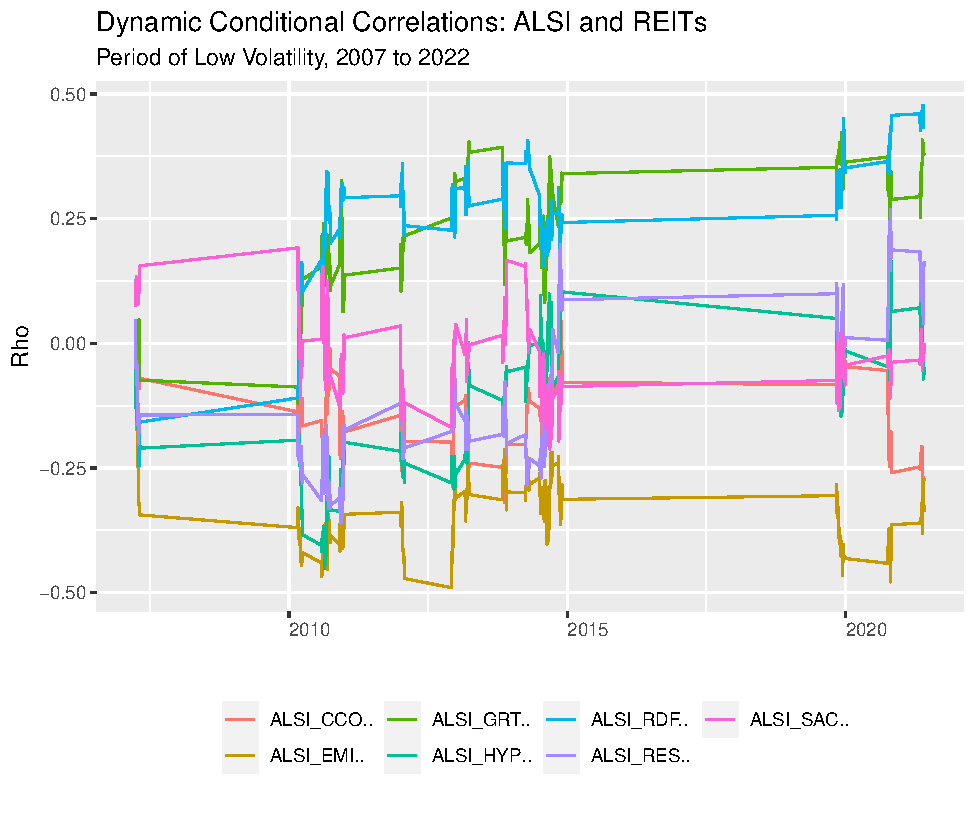
\includegraphics{Fin_Metrics_Project_files/figure-latex/unnamed-chunk-10-1.pdf}
\caption{Dynamic Conditional Correlations Graph}
\end{figure}

\begin{figure}
\centering
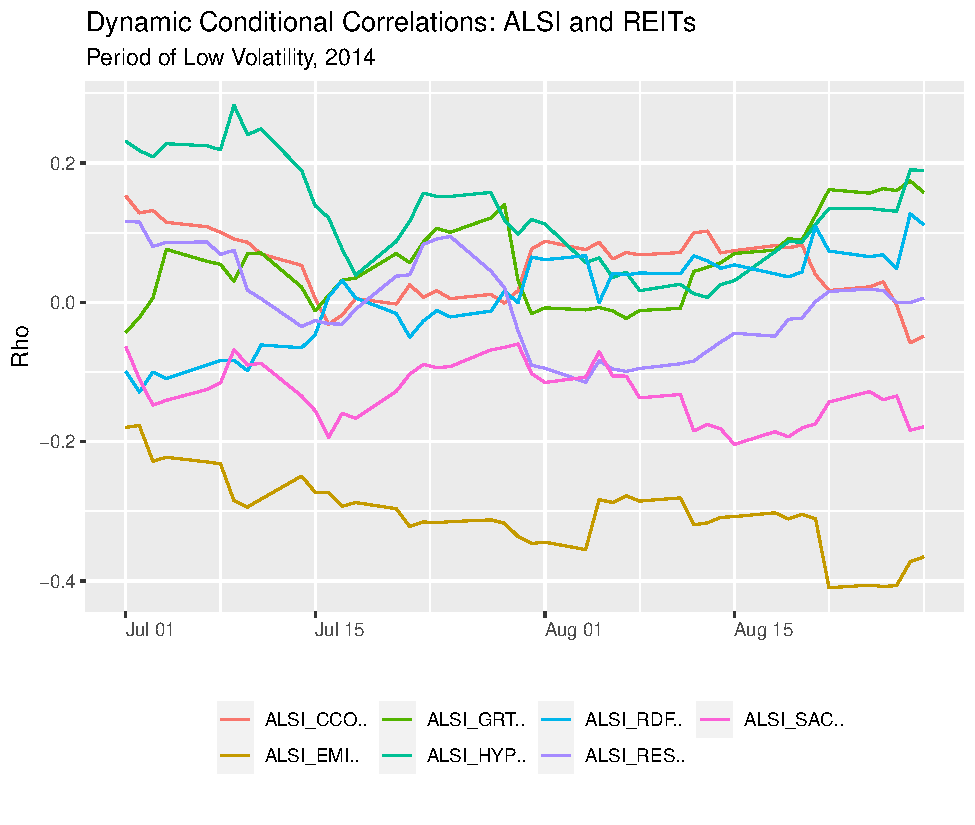
\includegraphics{Fin_Metrics_Project_files/figure-latex/unnamed-chunk-12-1.pdf}
\caption{Dynamic Conditional Correlations Graph}
\end{figure}

\hypertarget{time-varying-correlation-capco-vs-other-reits-and-alsi}{%
\subsection{Time-varying Correlation: Capco vs Other REITs and
ALSI}\label{time-varying-correlation-capco-vs-other-reits-and-alsi}}

\begin{figure}
\centering
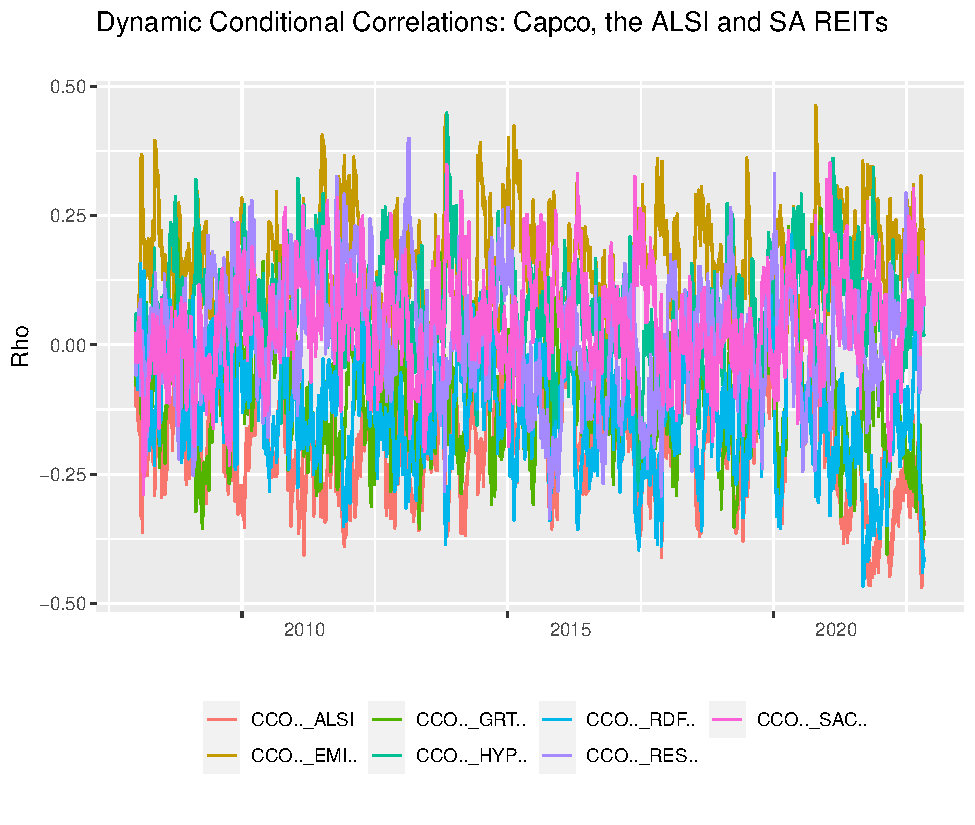
\includegraphics{Fin_Metrics_Project_files/figure-latex/unnamed-chunk-13-1.pdf}
\caption{Dynamic Conditional Correlations Graph}
\end{figure}

\begin{figure}
\centering
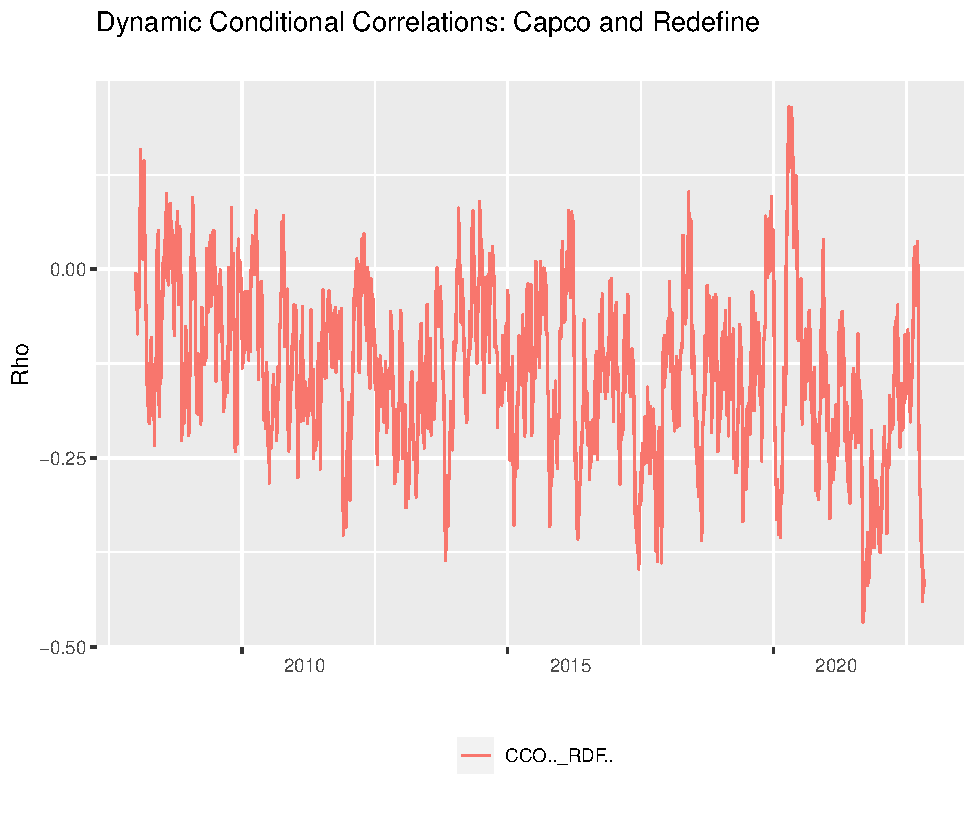
\includegraphics{Fin_Metrics_Project_files/figure-latex/unnamed-chunk-14-1.pdf}
\caption{Dynamic Conditional Correlations Graph}
\end{figure}

\hypertarget{conclusion}{%
\section{\texorpdfstring{Conclusion
\label{Conclusion}}{Conclusion }}\label{conclusion}}

\newpage

\hypertarget{references}{%
\section*{References}\label{references}}
\addcontentsline{toc}{section}{References}

Engle, R. (2002) Dynamic Conditional Correlation: A Simple Class of
Multivariate Generalized Autoregressive Conditional Heteroskedasticity
Models. Journal of Business \& Economic Statistics, 20, 339-350.

\bibliography{Tex/ref}





\end{document}
